\begin{figure}[h!]
    \centering
    \caption{Série temporal dos sensores de \acrshort{o3} modelo OX-B431}
    \begin{subfigure}{0.4\textwidth}
        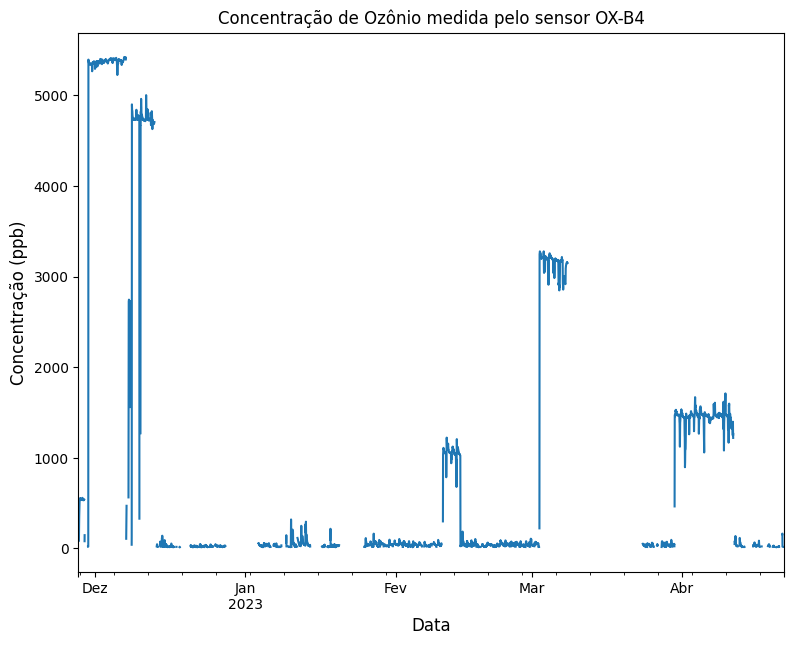
\includegraphics[width=\textwidth]{chapters/3-ANÁLISE DOS DADOS/Figuras/raw-o3-b4-1.png}
        \caption{Série temporal do sensor 1 depois de remover valores fora de intervalo}
        \label{fig:data-o3-1-raw}
    \end{subfigure}
    \hfill
    \begin{subfigure}{0.4\textwidth}
        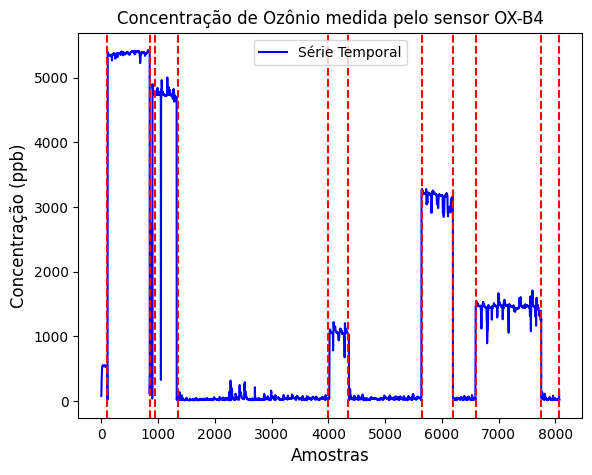
\includegraphics[width=\textwidth]{chapters/3-ANÁLISE DOS DADOS/Figuras/rebase-o3-b4-1.png}
        \caption{Pontos de alteração da linha base no sensor 1 detectados pelo algoritmo \acrshort{pelt}}
        \label{fig:data-rebase-o3-1}
    \end{subfigure}
    \hfill
    \begin{subfigure}{0.4\textwidth}
        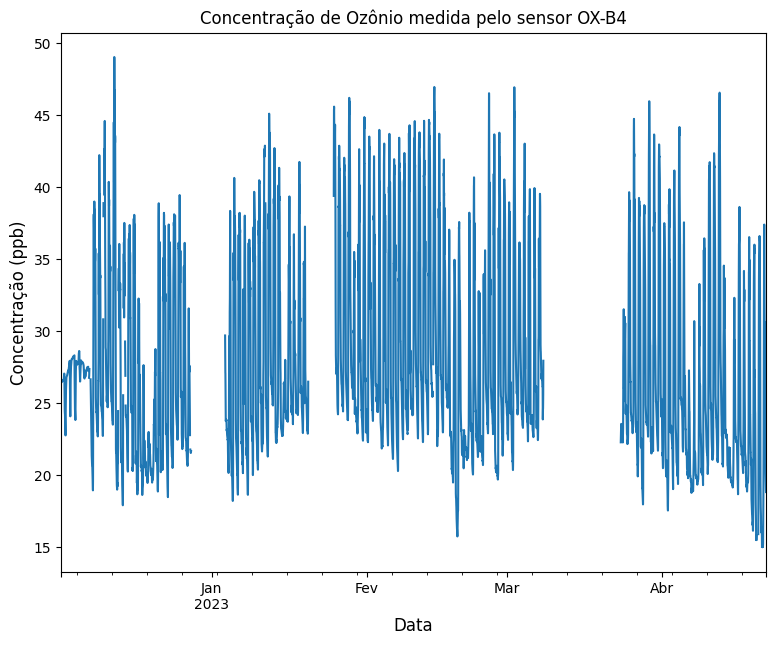
\includegraphics[width=\textwidth]{chapters/3-ANÁLISE DOS DADOS/Figuras/raw-o3-b4-2.png}
        \caption{Série temporal do sensor 2 depois de remover valores fora de intervalo}
        \label{fig:data-o3-2-raw}
    \end{subfigure}
    \label{fig:data-o3-raw-and-pelt}
\end{figure}

% ----------------------------------------------------------
\section{Análise dos dados de Ozônio}
% ----------------------------------------------------------

Para a medição de \acrshort{o3} foram utilizados dois sensores do modelo OX-B431. As Figuras \ref{fig:data-o3-1-raw} e \ref{fig:data-o3-2-raw} mostram as séries temporais dos sensores depois de removidos os valores fora de intervalo. Observa-se que o sensor 1 sofreu alterações no valor de linha base nos meses de dezembro, fevereiro, março e abril, que foram detectadas pelo algoritmo \acrshort{pelt}, conforme ilustrado na Figura \ref{fig:data-rebase-o3-1}. As amostras dentro dos intervalos que apresentaram variações na linha base no sensor 1 foram etiquetados correspondentemente para sua remoção. As leituras do sensor 2 não apresentaram alterações na linha base.

\begin{figure}[h!]
    \centering
    \caption{Séries temporais dos sensores OX-B431 pré-processadas}
    \begin{subfigure}{0.9\textwidth}
        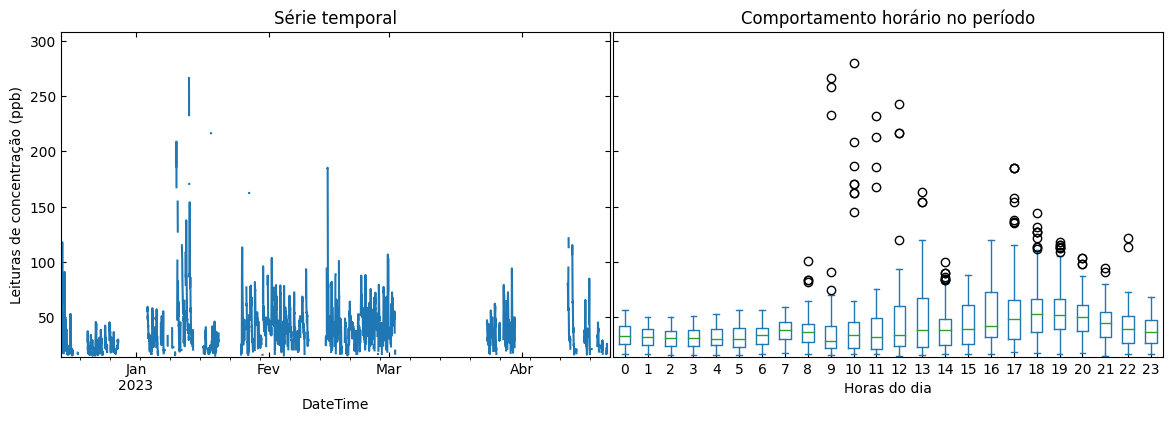
\includegraphics[width=\textwidth]{chapters/3-ANÁLISE DOS DADOS/Figuras/preproc-ox-b4-1.png}
        \caption{Série temporal do sensor 1 pré-processada (T = 15 mins) e seu comportamento diário}
        \label{fig:data-o3-1-preproc-15}
    \end{subfigure}
    \begin{subfigure}{0.9\textwidth}
        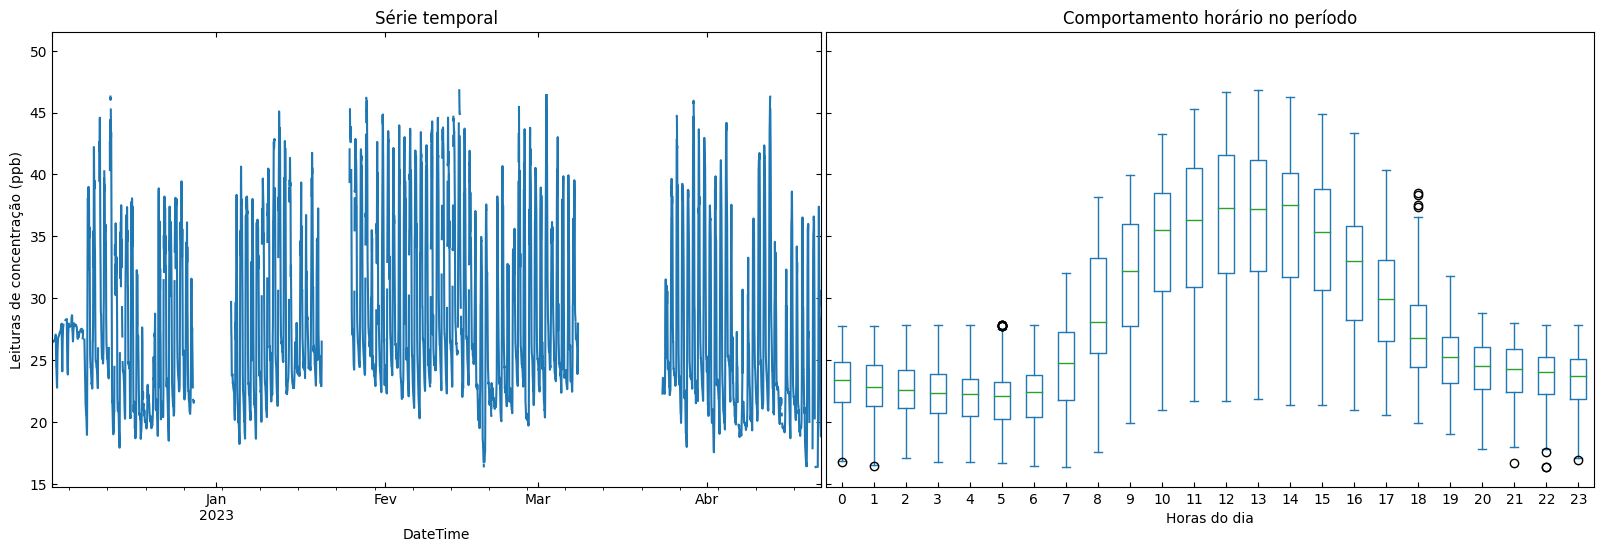
\includegraphics[width=\textwidth]{chapters/3-ANÁLISE DOS DADOS/Figuras/preproc-ox-b4-2.png}
        \caption{Série temporal do sensor 2 pré-processada (T = 15 mins) e seu comportamento diário}
        \label{fig:data-o3-2-preproc-15}
    \end{subfigure}
    \begin{subfigure}{0.9\textwidth}
        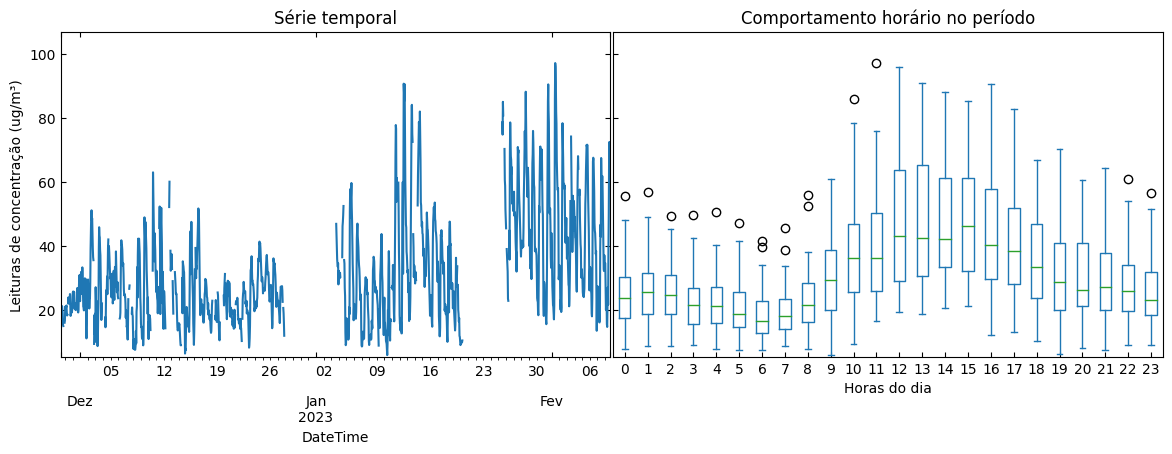
\includegraphics[width=\textwidth]{chapters/3-ANÁLISE DOS DADOS/Figuras/o3-reference-series-and-box.png}
        \caption{Série temporal das leituras de concentração de referência (T = 1 H) e seu comportamento diário}
        \label{fig:data-o3-reference}
    \end{subfigure}
    \label{fig:data-o3-preproc-15}
\end{figure}

Depois de pré-processadas as leituras dos sensores de ozônio obtiveram-se os resultados ilustrados nas Figuras \ref{fig:data-o3-1-preproc-15} e \ref{fig:data-o3-2-preproc-15}. Os gráficos mostram as séries dos dados pré-processados dos dois sensores OX-B431 juntamente com o comportamento diário das medições ao longo do período, agrupados por hora do dia. Na Figura \ref{fig:data-o3-reference} observa-se uma clara componente diária nas leituras de concentração, que coincide com o comportamento apresentado pelas medições de referência (Figura \ref{fig:data-o3-reference}). Esse comportamento é esperado nas medições de \acrshort{o3} já que a variável é influenciada pela luz solar.

\begin{table}[h!]
    \caption{Contabilização dos dados por etiquetas das leituras do sensor 1 OX-B431}
    \centering
    \begin{tabularx}{0.95\textwidth}[h]{
         >{\raggedright\hsize=.475\hsize\arraybackslash}X
         >{\raggedright\hsize=.20\hsize\arraybackslash}X 
         >{\raggedright\hsize=.5\hsize\arraybackslash}X
        | >{\raggedright\hsize=.50\hsize\arraybackslash}X 
         >{\raggedright\hsize=.20\hsize\arraybackslash}X 
         >{\raggedright\hsize=.5\hsize\arraybackslash}X }
        \multicolumn{3}{c|}{Série temporal T = 15 mins} & \multicolumn{3}{c}{Série temporal T = 1 hr} \\
        \hline
        Etiquetas & No. amostras & \% amostras & Etiquetas & No. amostras & \% amostras \\ [0.5ex]
        \hline
        \textit{MISSING} & 2750 & 18.80 \% & \textit{LOWSAMPLES} & 2020 & 65.67 \% \\ [0.5ex]
        
        \textit{LTLL} & 3134 & 21.43 \% & \textit{VALID} & 1056 & 34.33 \% \\ [0.5ex]
        
        \textit{GTUL} & 0 & 0.0 \% & & & \\ [0.5ex]
        
        \textit{STABILIZING} & 514 & 3.51 \% & & & \\ [0.5ex]
        
        \textit{BADSPIKE} & 56 & 0.38 \% & & & \\ [0.5ex]
        
        \textit{LTQTLE01} & 102 & 0.70 \% & & & \\ [0.5ex]
        
        \textit{GTQTLE99} & 64 & 0.44 \% & & & \\ [0.5ex]
        
        \textit{REBASE} & 3592 & 24.56 \% & & & \\ [0.5ex]

        \textit{VALID} & 4413 & 30.17 \% & & & \\ [0.5ex]
        \hline
        TOTAL & 14625 & & TOTAL & 3076 & \\
    \end{tabularx}
    \label{tab:data-contab-o3-1}
\end{table}

Histogramas das leituras dos sensores OX-B431 são mostrados nas Figuras \ref{fig:data-o3-1-preproc-hist} e \ref{fig:data-o3-2-preproc-hist}. Os dados adquiridos pelo sensor 1 apresentaram um comportamento log-normal. Já o sensor 2 produziu leituras com uma componente log-normal e uma outra componente de menor frequência nos valores de concentração acima 30 ppb. Esta última representa a componente com sazonalidade diária mencionada acima. As séries re-amostradas em períodos de 1 hora são mostradas nas Figuras \ref{fig:data-o3-1-preproc-1HR} e \ref{fig:data-o3-2-preproc-1HR}.

\begin{figure}[h]
    \centering
    \caption{Histogramas e séries temporais horárias das leituras dos sensores OX-B431}
    \begin{subfigure}{0.4\textwidth}
        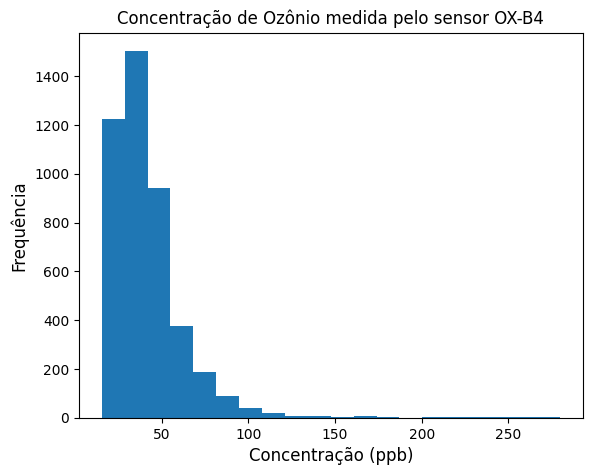
\includegraphics[width=\textwidth]{chapters/3-ANÁLISE DOS DADOS/Figuras/preproc-hist-ox-b4-1.png}
        \caption{Histograma das leituras do sensor 1 OX-B431}
        \label{fig:data-o3-1-preproc-hist}
    \end{subfigure}
    \hfill
    \begin{subfigure}{0.4\textwidth}
        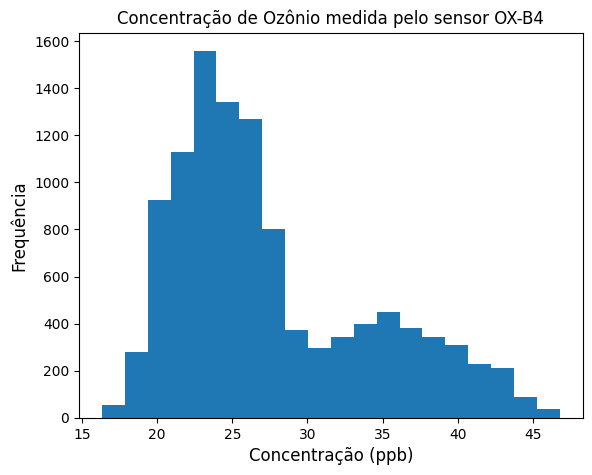
\includegraphics[width=\textwidth]{chapters/3-ANÁLISE DOS DADOS/Figuras/preproc-hist-ox-b4-2.png}
        \caption{Histograma das leituras do sensor 2 OX-B431}
        \label{fig:data-o3-2-preproc-hist}
    \end{subfigure}
    \hfill
    \begin{subfigure}{0.4\textwidth}
        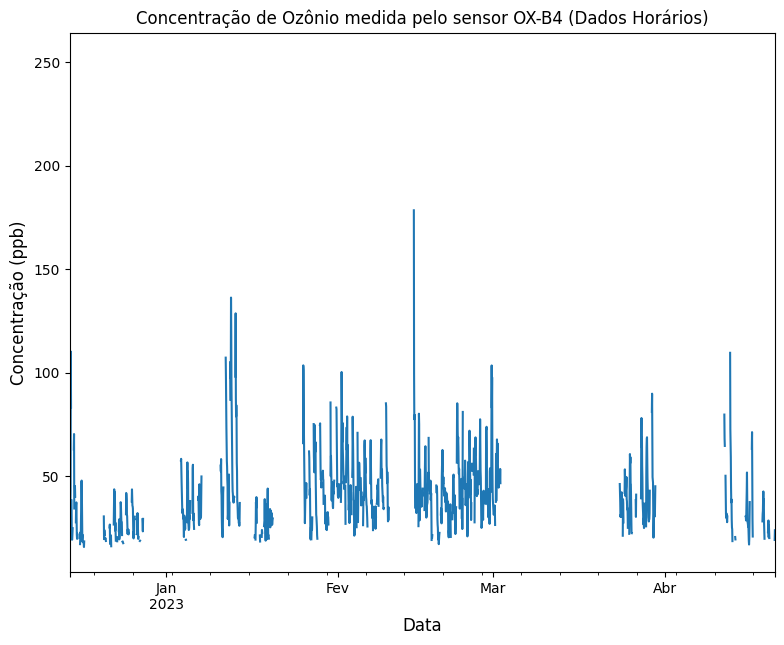
\includegraphics[width=\textwidth]{chapters/3-ANÁLISE DOS DADOS/Figuras/preproc-1HR-ox-b4-1.png}
        \caption{Série temporal do sensor 2 com T = 1 hr}
        \label{fig:data-o3-1-preproc-1HR}
    \end{subfigure}
    \hfill
    \begin{subfigure}{0.4\textwidth}
        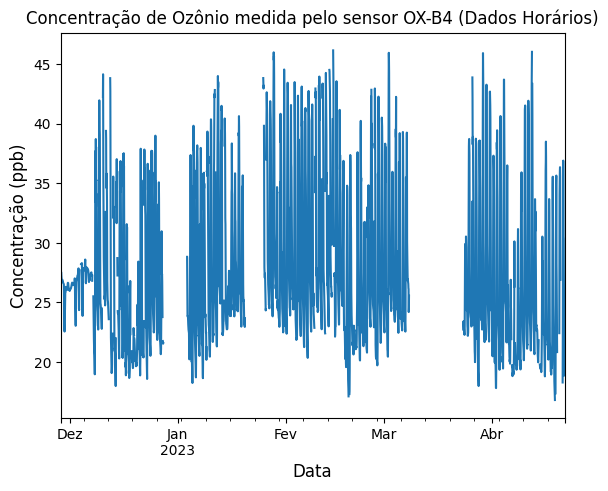
\includegraphics[width=\textwidth]{chapters/3-ANÁLISE DOS DADOS/Figuras/preproc-1HR-ox-b4-2.png}
        \caption{Série temporal do sensor 2 com T = 1 hr}
        \label{fig:data-o3-2-preproc-1HR}
    \end{subfigure}
\end{figure}

Nas Tabelas \ref{tab:data-contab-o3-1} e \ref{tab:data-contab-o3-2} contabilizam-se os dados dos sensores de \acrshort{o3} para períodos de 15 minutos e de 1 hora. Observa-se que no sensor 1, dos 14625 pontos de dados, que representavam as amostras adquiridas com um período de 15 minutos no intervalo de 20/11/2022 até 21/04/2023, 4413 foram aproveitados como dados válidos, o que representa um 30 \% aproximadamente dos dados originais. Ao re-amostrar esses 4413 pontos em dados horários obtiveram-se 1056 amostras horárias de concentração válidas (aproximadamente 34 \% dos dados) para realizar a calibração. Já no sensor 2, dos 14542 pontos de dados, que representavam as amostras adquiridas no intervalo de 21/11/2022 até 21/04/2023, 10814 foram aproveitados como dados válidos, o que representa um 74 \% aproximadamente dos dados originais. Ao re-amostrar esses 10814 pontos válidos em dados horários obtiveram-se 2685 amostras horárias de concentração válidas (aproximadamente 77 \% dos dados) para realizar a calibração.

\begin{table}[h!]
    \caption{Contabilização dos dados por etiquetas das leituras do sensor 2 OX-B431}
    \centering
    \begin{tabularx}{0.95\textwidth}[h]{
         >{\raggedright\hsize=.475\hsize\arraybackslash}X
         >{\raggedright\hsize=.20\hsize\arraybackslash}X 
         >{\raggedright\hsize=.5\hsize\arraybackslash}X
        | >{\raggedright\hsize=.50\hsize\arraybackslash}X 
         >{\raggedright\hsize=.20\hsize\arraybackslash}X 
         >{\raggedright\hsize=.5\hsize\arraybackslash}X }
        \multicolumn{3}{c|}{Série temporal T = 15 mins} & \multicolumn{3}{c}{Série temporal T = 1 hr} \\
        \hline
        Etiquetas & No. amostras & \% amostras & Etiquetas & No. amostras & \% amostras \\ [0.5ex]
        \hline
        \textit{MISSING} & 2734 & 18.80 \% & \textit{LOWSAMPLES} & 783 & 22.58 \% \\ [0.5ex]
        
        \textit{LTLL} & 49 & 0.34 \% & \textit{VALID} & 2685 & 77.42 \% \\ [0.5ex]
        
        \textit{GTUL} & 0 & 0.0 \% & & & \\ [0.5ex]
        
        \textit{STABILIZING} & 673 & 4.63 \% & & & \\ [0.5ex]
        
        \textit{BADSPIKE} & 0 & 0.0 \% & & & \\ [0.5ex]
        
        \textit{LTQTLE01} & 125 & 0.86 \% & & & \\ [0.5ex]
        
        \textit{GTQTLE99} & 147 & 1.01 \% & & & \\ [0.5ex]
        
        \textit{REBASE} & 0 & 0.0 \% & & & \\ [0.5ex]
        
        \textit{VALID} & 10814 & 74.36 \% & & & \\ [0.5ex]
        \hline
        TOTAL & 14542 & & TOTAL & 3468 & \\
    \end{tabularx}
    \label{tab:data-contab-o3-2}
\end{table}

\subsection{Dependência com a temperatura}

Investigou-se a existência de correlação entre as leituras dos sensores de \acrshort{o3} e as variações de temperatura medida no interior da câmara de medição. Os resultados dos testes estatísticos de Spearman e Kendall revelaram coeficientes de correlação significativos, conforme se ilustra nas Figuras \ref{fig:data-temp-o3-1-corr} e \ref{fig:data-temp-o3-2-corr}. Os coeficientes de Spearman calculados foram de 0.37 e 0.85 para os sensores 1 e 2 respectivamente, com valores de p inferiores a 0.05, indicando uma correlação estatisticamente significativa entre as leituras dos sensores e a temperatura. De maneira semelhante, os coeficientes de Kendall foram de 0.27 e 0.70 respectivamente, também com p < 0.05, reforçando a presença de uma associação significativa. Ao avaliar a hipótese nula de ausência de correlação, os resultados forneceram evidências para sua rejeição, sugerindo a existência de uma correlação entre as leituras dos sensores de \acrshort{o3} e as variações de temperatura.

\begin{figure}[h!]
    \centering
    \caption{Relação entre as leituras dos sensores de \acrshort{o3} e a temperatura}
    \begin{subfigure}{0.495\textwidth}
        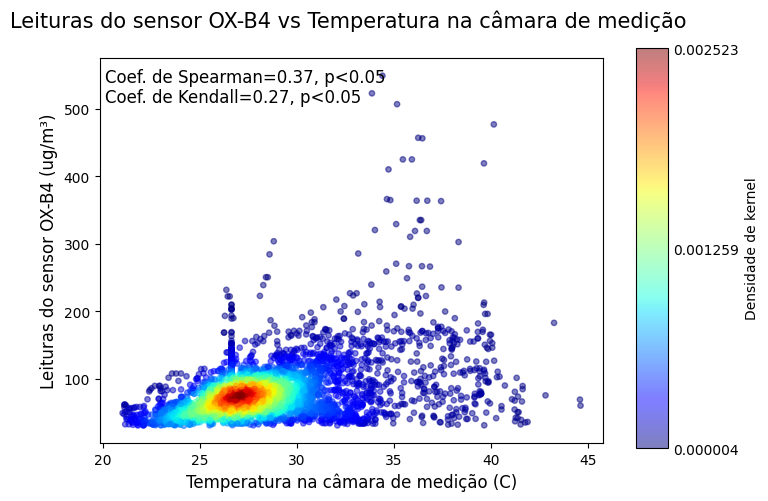
\includegraphics[width=\textwidth]{chapters/3-ANÁLISE DOS DADOS/Figuras/temperature-o3-b4-1.png}
        \caption{Relação entre as leituras do sensor 1 de \acrshort{o3} e a temperatura}
        \label{fig:data-temp-o3-1-corr}    
    \end{subfigure}
    \hfill
    \begin{subfigure}{0.495\textwidth}
        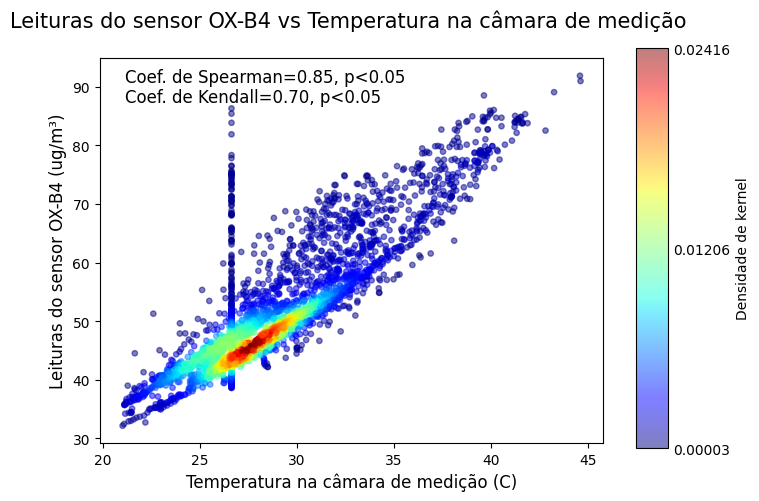
\includegraphics[width=\textwidth]{chapters/3-ANÁLISE DOS DADOS/Figuras/temperature-o3-b4-2.png}
        \caption{Relação entre as leituras do sensor 2 de \acrshort{o3} e a temperatura}
        \label{fig:data-temp-o3-2-corr}    
    \end{subfigure}
    \hfill
    \begin{subfigure}{0.495\textwidth}
        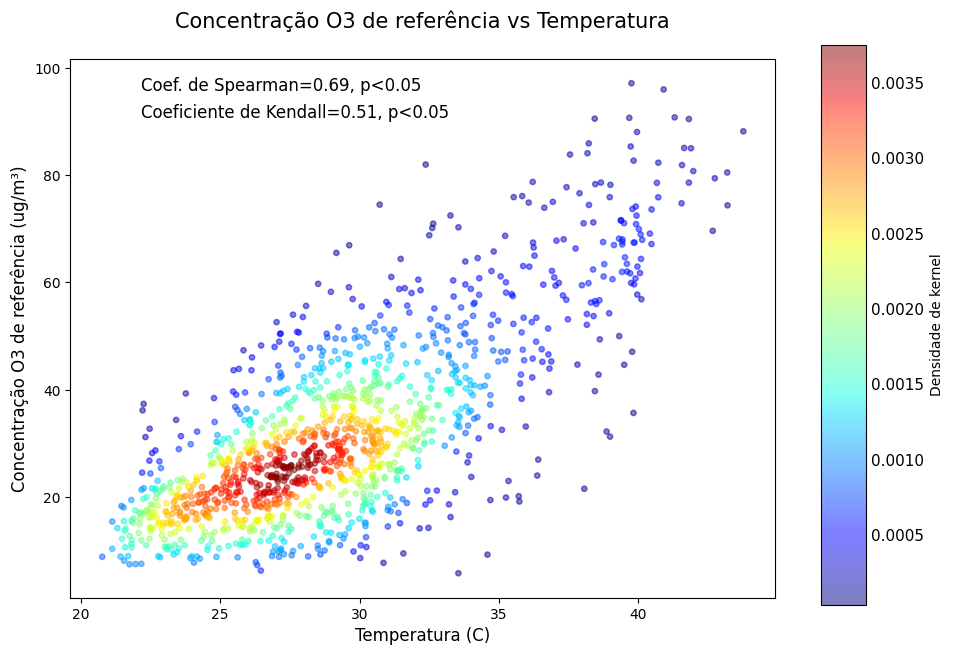
\includegraphics[width=\textwidth]{chapters/3-ANÁLISE DOS DADOS/Figuras/temperature-o3-reference.png}
        \caption{Relação entre os valores de concentração de referência e a temperatura}
        \label{fig:data-temp-o3-ref-corr}    
    \end{subfigure}
    \label{fig:data-temp-o3-corr}
\end{figure}

Os resultados obtidos nos testes estatísticos podem ser corroborados nos gráficos de dispersão entre as variáveis nas Figuras \ref{fig:data-temp-o3-1-corr} e \ref{fig:data-temp-o3-2-corr}. Delas comprova-se uma maior correlação com a temperatura no sensor 2, que coincide com o comportamento sazonal diário observado anteriormente. As leituras de referência também apresentaram uma relação linear com a temperatura, com coeficientes de Spearman e Kendall de 0.69 e 0.51 respectivamente, conforme se ilustra na Figura \ref{fig:data-temp-o3-ref-corr}.

% ----------------------------------------------------------
\subsection{Comparação das leituras dos sensores OX-B431 com as medições de referência}
% ----------------------------------------------------------

Nas Figuras \ref{fig:data-o3-reference-time-series}, \ref{fig:data-o3-1-reference-corr} e \ref{fig:data-o3-2-reference-corr} apresentam-se as leituras de \acrshort{o3} obtidas pelos sensores OX-B431 de Alphasense e a estação de referência. Observa-se que as leituras do sensor 1 superestimaram os valores de concentração de referência. Os testes de Spearman e Kendall revelaram a existência de correlação entre as medições com o sensor 1 e a referência com coeficientes de 0.38 e 0.27 respectivamente, e de 0.59 e 0.42 respectivamente para o sensor 2.

\begin{figure}[h]
    \centering
    \caption{Séries temporais e gráficos de dispersão das medições de \acrshort{o3}}
    \begin{subfigure}{0.4\textwidth}
        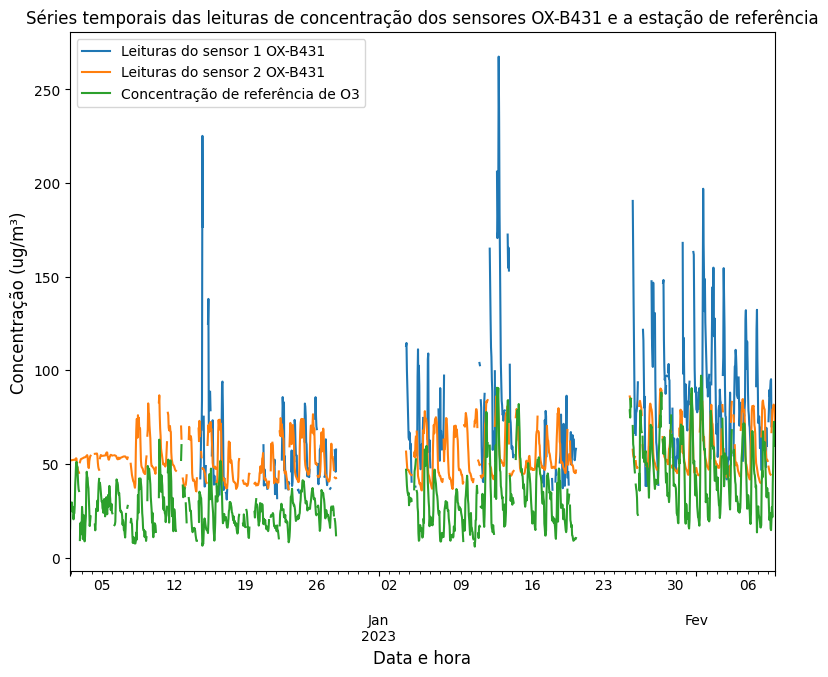
\includegraphics[width=\textwidth]{chapters/3-ANÁLISE DOS DADOS/Figuras/o3-b4-reference-time-series.png}
        \caption{Séries temporais das leituras dos sensores OX-B431 e a estação de referência}
        \label{fig:data-o3-reference-time-series}
    \end{subfigure}
    \hfill
    \begin{subfigure}{0.5\textwidth}
        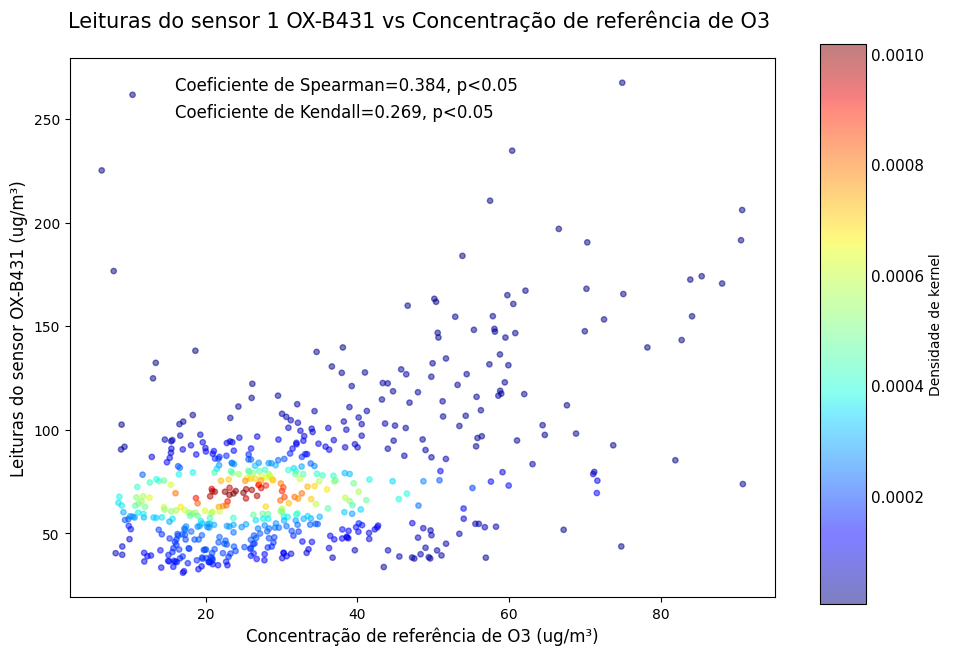
\includegraphics[width=\textwidth]{chapters/3-ANÁLISE DOS DADOS/Figuras/o3-b4-1-reference-correlation.png}
        \caption{Gráfico de dispersão das leituras do sensor 1 OX-B431 e a estação de referência}
        \label{fig:data-o3-1-reference-corr}
    \end{subfigure}
    \hfill
    \begin{subfigure}{0.5\textwidth}
        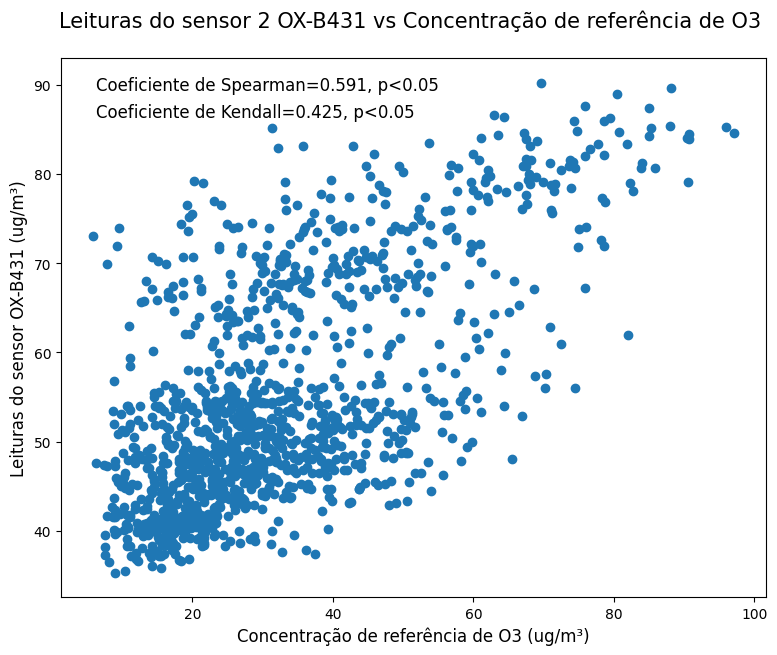
\includegraphics[width=\textwidth]{chapters/3-ANÁLISE DOS DADOS/Figuras/o3-b4-2-reference-correlation.png}
        \caption{Gráfico de dispersão das leituras do sensor 2 OX-B431 e a estação de referência}
        \label{fig:data-o3-2-reference-corr}
    \end{subfigure}
\end{figure}